\chapter{Scalable Type Inferencing}

Authors: Michael Wilder, Anthony Jones and Clinton Jeffery

\bigskip

This chapter details compile-time space savings in iconc that enable
it to handle large Unicon programs.  The Icon compiler represents all
the possible types as a bit vector with each bit position representing
a specific type. Such vectors are required for each variable including
each temporary variable location as a result of subexpression
evaluation. The type inferencing model allocates a unique type to each
source location at which heterogeneous structure types such as lists
or records are created.  In the course of compiling a large program,
the number of total types, and therefore the size of the bit vectors,
can skyrocket. According to Walker [Walker93],
the type inferencer described in Chapters
15 and 19 has a space cost of $O(n^{3})$.
The associated constants, and the value of n, may be
large. Improving the memory usage of iconc's type inferencing system
was necessary because the compiler was empirically observed to run out
of memory compiling large programs.

At the time it was developed, iconc was able to compile small to
medium size Icon programs. Although main memories in typical computers
have increased from 4MB to 4GB in the years since iconc was developed,
Unicon programs can be much larger than Icon programs. Likewise,
heavily object-oriented programs, such as ones with graphical user
interfaces, are especially demanding for the type inferencer, as they
introduce large numbers of new types. For these reasons, the space
needed for type inferencing was a problem that demanded attention
and limited the applicability of the optimizing compiler.

In 1996 Anthony Jones introduced compact representations that reduced
space requirements by approximately a factor of 3 [Jones96],
providing enough relief to allow iconc to compile some larger programs
of the time.  These improvements were subsumed a decade later by the
work described in this chapter. After realizing that type information
was frequently duplicated, a type vector hashing scheme was introduced
by which almost all redundant allocations of type information were
avoided. This work effectively solved the memory space scalability
problem for type inferencing.


\section{The Type Representation}

One way to reduce space requirements is to optimize the representation
of type information. Iconc maintains a structure for each variable
that contains information about that variable, including a bit vector
with each bit representing a particular type used in the program. When
a bit vector is allocated it is one of three possible sizes. The first
size is composed of first class types which are those built in types
plus user defined types that are utilized. The second size consists of
the first class types plus intermediate value types. Lastly, there is
the number of total types in the database. The database refers to the
collection of all builtin operations, their number of parameters and
types, and the type for the return value.

Data was gathered from \textit{Ctree}, a circular tree visualization
tool. This program consists of \~{}500 lines of source code. The
number of possible first class types is 209 which translates to a 28
byte bit vector. Note that bit vectors are allocated in multiples of a
word (4 bytes). During the course of the compilation, 137,946 bit
vectors are allocated. The number of first class types plus types for
intermediate values is 1,012, resulting in a 128 byte bit vector, and
18,925 vectors of this size are allocated. Lastly, the number of
database types is 1,369 types, using a 172 byte bit vector with only
121 allocations of this size. The total memory requirement for the bit
vectors is 6.22 megabytes. This information is summarized in Figure
24-1.

\begin{center}
\tablefirsthead{\hline
{\itshape Vector Type} &
{\itshape Number of Types} &
{\itshape Number Allocated} &
{\itshape Required Memory (MB)}\\}
\tablehead{\hline
{\itshape Vector Type} &
{\itshape Number of Types} &
{\itshape Number Allocated} &
{\itshape Required Memory (MB)}\\}
\tabletail{}
\tablelasttail{}
\begin{xtabular}{|m{1.2191598in}|m{1.1629599in}|m{1.2455599in}|m{1.6080599in}|}
\hline
 first class &
\raggedleft 209 &
\raggedleft 137946 &
\raggedleft\arraybslash 3.8\\\hline
 intermediate class &
\raggedleft 1012 &
\raggedleft 18925 &
\raggedleft\arraybslash 2.4\\\hline
 database class &
\raggedleft 1369 &
\raggedleft 121 &
\raggedleft\arraybslash 0.02\\\hline
\end{xtabular}
\end{center}
{\centering\selectlanguage{english}
Figure 24-1: Bit Vector Sizes
\par}


Figure 24-2 is an example of what a bit vector from \textit{Ctree}
might look like. This example shows the division between the three
type classes. Within the partition for first class types is bit 0
which represents an integer and bit 6 which is a real. Within the
intermediate types partition, bit 209 represents an instance of a
\texttt{cnode} record and an instance of a list variable, and bit 232
is an instance of a variable that is of the list type. Every instance
of a list or an aggregate type such as a record results in a new type
that gets its own bit in the bit vector.

Lastly, within the database class are builtin operations. The
functions for random number (\texttt{O0z7\_random}) and subtraction
(\texttt{O114\_subc}) are assigned bits 1,012 and 1,368
respectively. The functions are builtin to the Icon compiler and are
assigned their own types in the bit vector.

\bigskip

\begin{center}
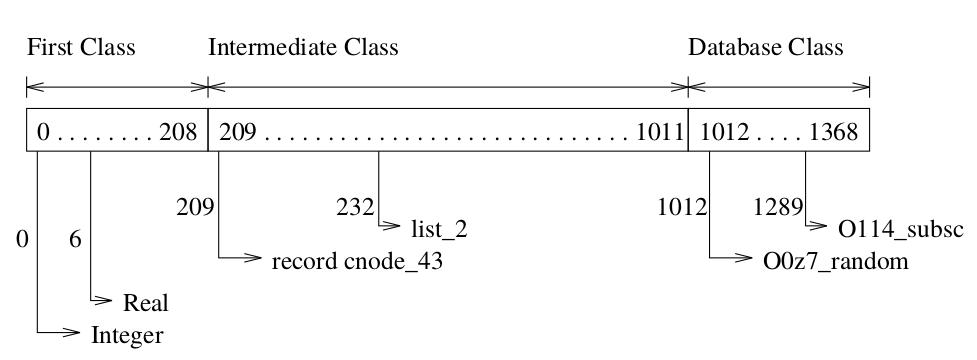
\includegraphics[width=6.0in,height=2.2in]{bit_sizes.png}

Figure 24-2: Sample Bit Vector
\end{center}

Additional tests were run on a 25,000 line Icon (really Idol) program
called \textit{Freedom in the Galaxy}, which was a semester long
effort by Dr. Jeffery's Software Engineering class. The program has
hundreds of variables, but object-orientation requires many additional
intermediate variables and dramatically increases the number and
size of type vectors allocated during compilation. \textit{Freedom in
the Galaxy} has 12,591 different distinct types including builtin,
intermediate, and database types. This is an example of a program that
ran out of memory during compilation with iconc on typical
workstations in the mid-1990's, motivating space improvements.

\section{Type Vector Hashing}

Type inferencing in iconc uses collections of large bit vectors that
are frequently referenced. The bit vectors represent sets of possible
types at each program point. This section presents an incremental
technique that dramatically reduces the space required for these bit
vectors. The technique depends on a classic data structure: the hash table.

Hash tables are used in many different application domains to map keys
(usually small) onto (often much larger) values. In their degenerate
form, hash tables can be used to store a set of keys, with no
associated values. Such sets may be needed for purposes of memory
sharing, as in the Flyweight design pattern. The traditional hash
table {\textit{O}}(1) average case lookup and insert speeds break down
when the keys are very large (for example, hundreds of machine words)
and heavily referenced (many millions or billions of lookups). In such
circumstances, it is imperative to identify a fast hash function that
performs well despite the large data keys to be hashed.

\section{Type Inferencing}

As mentioned previously, iconc's type inferencer originally required
\textit{O}(n\textsuperscript{2}) space on average and
\textit{O}(n\textsuperscript{3}) in the worst case, where n
corresponds to program size (as a number of expressions, not bytes or
lines of code).  The inferencer allocated large bit vectors at every
(sub)expression point in a program where typed values are
transmitted. This algorithm runs acceptably for small and medium size
programs, but fails for large programs. For example, in one of the
test programs, the brute force algorithm attempted to
\textsf{malloc()} 24GB of memory, exceeding the capacity of the test
machine. By the time such allocations are easily supported on most
computers, larger Unicon programs will be written for which even more
space will be needed. Type inferencing
space requirements are exacerbated in object-oriented programs which
may utilize many hundreds of user-defined types for classes and their
method vectors.

\section{A Copy-on-Write Type Vector Pool}

Analysis revealed much redundancy among type vectors associated with
type-mutable program points when inferring the types in
programs. Hashing was introduced to eliminate type vector redundancy
by employing copy-on-write semantics in a type vector pool. Using a
hash table to implement a shared pool of bit vectors largely solves
the space problem, reducing space needs to \textit{O}(n) on average
and \textit{O}(n\textsuperscript{2}) in the worst case, at a
potentially large cost in time. If the time constants involved
increase the real-world time to an impractical extent, then the use of
hashing fails despite its successful space reduction.

The hashing of type vectors in the type inferencer poses many
challenges. The width of type vectors varies with the number of
run-time types present in an input program. Type vectors in the type
inferencer can be quite large because the run-time type information
produced is of very high quality. For example, in addition to bits for
all the base types and declared record or class types, the bit vector
also must contain bits for each field (or member variable) of each
class or record. The type inferencer also uses a separate bit in the
vector to differentiate each constructor site for composite types
(such as lists). A list containing strings, for instance, is assigned
a different type than a list containing records or a list containing
strings and records. This fine granularity of type information
contributes admirably to the speedup of targets generated by the
Unicon Compiler, but causes type vectors to become very large during
type inferencing.

The number of vectors required for type inferencing depends upon the
number of type-mutable program points in the dataflow graph of the
input program. Some programs have many possible types, but contain
relatively few type-mutable program points; other programs contain
relatively few run-time types but have many type-mutable program
points. And, of course, some programs contain many type-mutable
program points and many possible run-time types. These variables
exacerbate the requirements imposed upon a type vector hashing
scheme. To add further interest, analysis of the bit patterns held in
non-redundant type vectors within the type inferencer at compile-time
revealed no reliable lever of disparity that could be employed as a
collision reductive agent in a type vector hashing scheme.

\section{Implementation}

Implementation began with a software harness to permit the direct
comparison of various hashing techniques within the specific confines
of the Unicon Compiler type inferencer. Experimentation produced a
fixed-address, multiplicative hashing scheme wherein the number of
buckets in the hash table is a variant power of 2 greater than
255. This number varies depending upon characteristics of the input
program ascertained before the start of type inferencing.

Type vectors are allocated from a pool of vectors that serves as the
vector store during type inferencing. The size of this pool also
varies depending upon characteristics of the input program ascertained
before the start of type inferencing. The pool of vectors contained in
the Unicon Compiler type inferencer is a discrete entity that is not
accessed directly by the type vector hash table. This separation
facilitates experimentation with different pooling algorithms and
implementations without modifying the type vector hash table
implementation. All pools in the Unicon Compiler type inferencer are
implemented in this manner.

The vector hash table implementation in the Unicon Compiler does not
permit the migration of type vectors among buckets in the hash
table. Once a type vector is inserted into a hash table bucket, it
remains in situ for the duration of type inferencing. Reference counts
are not maintained for type vectors contained within the hash table
because any type vector in the system (except one) is created as the
result of a transformation applied to another type vector that already
exists within the type vector hash table.

A tremendous savings of space during type inferencing was immediately
realized by eliminating type vector redundancy through hashing. The
initial space reductions obtained were comparable to those indicated
in Section 5. Although adding a hash table increases the complexity
and likewise increases the number of instructions required for type
vector generation, eliminating type vector redundancy provided a
speedup of some vector manipulation operations because we were able to
employ reference-based vector equality comparisons where value-based
comparisons were previously required.

\subsection{Bit Vector Hashing}

An early version of the vector hashing function employed in the Unicon
Compiler type inferencer is depicted in Figure 24-6.  Subsequent analysis
and refinement of our hashing scheme produced a much faster method
than this straightforward approach.

\begin{iconcode}
00. static \\
01. inline \\
02. unsigned int \\
03. hash(bits) \\
04. \ \ \ \ \ unsigned int * bits; \\
05. \{ \\
06. \ \ \ \ \ int i; \\
07. \ \ \ \ \ unsigned long long rawhash, xor; \\
08. \ \ \ \ \ unsigned int cookedhash; \\
09. \\
10. \ \ \ \ \ rawhash = xor = 0ULL; \\
11. \ \ \ \ \ i = n\_rttyp\_ints - 1; \\
12. \ \ \ \ \ while (i {\textgreater}= 0) \{ \\
13. \ \ \ \ \ \ \ \ \ rawhash += xor; \\
14. \ \ \ \ \ \ \ \ \ rawhash += bits[i]; \\
15. \ \ \ \ \ \ \ \ \ xor \^{}= bits[i]; \\
16. \ \ \ \ \ \ \ \ \ i-{}-; \\
17. \ \ \ \ \ \ \ \ \ \} \\
18. \ \ \ \ \ rawhash *= 0x20c49ba5e353f7cfULL; \\
19. \ \ \ \ \ i = hash\_shifts; \\
20. \ \ \ \ \ cookedhash = rawhash \& hash\_mask; \\
21. \ \ \ \ \ while (i) \{ \\
22. \ \ \ \ \ \ \ \ \ rawhash {\textgreater}{\textgreater}= hash\_upper\_shr; \\
23. \ \ \ \ \ \ \ \ \ cookedhash \^{}= rawhash; \\
24. \ \ \ \ \ \ \ \ \ i-{}-; \\
25. \ \ \ \ \ \ \ \ \ \} \\
26. \ \ \ \ \ return (cookedhash \& hash\_mask); \\
27. \}
\end{iconcode}

{\centering Figure 24-6: Hashing before halving
\par}

In function \textsf{hash()}, the cumulative \textsf{xor} is used to
perturb the raw hash value. The variable \textsf{n\_rttyp\_ints} is
the size of array in words; \textsf{hash\_shifts} is the word size
divided by the bucket size, and is used in order to ensure that the
entire hash number is involved in bucket selection. The hex constant
was derived experimentally to maximize distribution on a wide range of
input bit vectors.

Having achieved a dramatic space reduction, the next step was to
refine the hashing and pooling algorithms to improve the speed of type
vector creation and retrieval during type inferencing.

\subsection{Hash Halving}

It is not uncommon to encounter type vectors that are well over 100
machine words wide when inferring the types of large
programs. Locality is a major performance impediment when hashing type
vectors in programs of this nature. The techniques described in this
section were devised to improve the speed of type inferencing in the
Unicon Compiler.

The hashing routine depicted in Figure 24-6 was employed in early
space-reduction experiments with the Unicon Compiler type
inferencer. This hashing routine traverses the entire length of a type
vector in order to compute its hash value. This conservative approach
makes use of all the information contained within the bits of a type
vector, but it becomes problematic when type vectors are hundreds of
machine words wide and the hashing routine is invoked hundreds of
millions of times during type inferencing. Approaches in which the
hash function considers only a portion of the information in a type
vector would hash faster, at the expense of more collisions. Instead,
we conducted experiments to reduce the time required to compute the
hash value of full type vectors. This experimentation produced a
technique referred to as {\textit{hash halving}}.

Hash halving permits the hashing of arbitrarily wide type vectors
without traversing said vectors. To accomplish this, the hashing
routine is split into a {\textit{top half}} routine and
{\textit{bottom half}} routine. The top half routine performs a full
traversal of a given type vector in order to produce a ``raw'' hash
value for the vector. The bottom half routine is a scrambling function
that transforms the raw hash value produced by the top half into a
``cooked'' hash value for the vector. Referring to the hashing routine
in Figure 1, lines 10-17 constitute the top half and lines 18-26
constitute the bottom half of this routine. In a conventional hashing
scheme, computing the hash value of a type vector would entail
invoking the top half and bottom half hashing routines. The Unicon
Compiler type inferencer does not do this.

It is immediately apparent that the bottom half of the hashing routine
in Figure 24-6 is computationally much less expensive than the top half
when type vectors are very wide. Lines 10-17 are executed in time
proportional to the width of the type vector being hashed, which in
the worst case is {\textit{O}}(n). Lines 18-26, on the other hand, are
{\textit{O}}(1) because the value of {\textsf{hash\_shifts}} will
never be larger than the width of a ``raw'' hash value. If, for
instance, a raw hash value is represented in 64 bits and the hash
table contains 256 buckets, the value of hash\_shifts is initialized
to 7 at the start of type inferencing. The intuition behind hash
halving is to circumvent the computational expense of the top half
whenever possible, thereby reducing the {\textit{O}}(n) cost of the
top half to an {\textit{O}}(1) incremental cost whenever a type vector
is modified. In the Unicon Compiler type inferencer, this is
facilitated by the fact that all type vectors instantiated during type
inferencing are descendants of a single type vector called the
{\textit{genesis vector}}.

At the start of type inferencing in the Unicon Compiler, there exists
a single type vector in the system. This genesis vector represents the
union of all types permissible in the input program. All type-mutable
program points in the dataflow graph of the input program initially
refer to this genesis vector because reference-based semantics are
used and no refinement of information about the types at said program
points has yet been accomplished. When the genesis vector is created
at the start of type inferencing, the raw (top half) hash value for
this vector is computed and stored as a datum with the vector. Any
subsequent vectors produced as a result of some transformation of this
genesis vector use the raw hash value stored in the genesis vector to
compute what the raw hash value of the potentially new type vector
would be, based upon the transformation applied to the genesis
vector. This computation occurs without any knowledge of the actual
content of the genesis vector.

The raw hash value associated with a type vector in the Unicon
Compiler type inferencer is a simple summation (see Figure 24-7). This
summation facilitates incrementality by permitting fast updating of
the raw hash value of a vector when attempting to determine the raw
hash value for a potentially new type vector.

For example, assume that some type-mutable program point contains a
reference to the genesis vector V {\TextSubscript{G}}. In the event
that the type inferencer wants to apply transform t{\TextSubscript{1}}
to V{\TextSubscript{G}}, it is desirable to determine whether the
result of this transformation (V{\TextSubscript{1}}) is already a
member of the vector hash table without performing a full hash of
V{\TextSubscript{1}. The Unicon Compiler type inferencer accomplishes
this as follows.

The raw hash value of V{\TextSubscript{G}} is copied into a temporary
vector. This raw hash value is then transformed {\textit{in place}}
based upon the nature of the transform t{\TextSubscript{1}} to produce
the raw hash value of the subject vector V{\TextSubscript{1}}. This
circumvents a call to the top half hashing routine. The type
inferencer then invokes the bottom half hashing routine to transform
the raw hash value of V{\TextSubscript{1}} into the cooked hash value
of V{\TextSubscript{1}}. If the vector hash table bucket corresponding
to the cooked hash value of V{\TextSubscript{1}} is empty,
V{\TextSubscript{1}} of course does not exist in the hash table.  The
temporary vector is populated with the content of the vector
V{\TextSubscript{G}}, the contents of the temporary vector are
transformed via t{\TextSubscript{1}}, and the temporary vector is
inserted into the vector hash table to become
V{\TextSubscript{1}}.

In the event that the vector hash table bucket corresponding to the
cooked hash value of the subject vector V{\TextSubscript{1}} is not
empty, the temporary vector is populated with the characteristics of
V{\TextSubscript{1}} and the hash table bucket is searched for the
subject vector V{\TextSubscript{1}}.


\bigskip

\begin{iconcode}
static inline unsigned long long hash\_th(bits) \\
\ \ \ \ unsigned int * bits; \\
\{ \\
\ \ \ \ int i; \\
\ \ \ \ unsigned long long h; \\
\ \ \ \ h = 0ULL; \\
\ \ \ \ i = n\_rttyp\_ints - 1; \\
\ \ \ \ while (i {\textgreater} 0) \{ \\
\ \ \ \ \ \ \ \ h += bits[i] * i; \\
\ \ \ \ \ \ \ \ i-{}-; \\
\ \ \ \ \ \ \ \ \} \\
\ \ \ \ h += bits[0]; \\
\ \ \ \ return h; \\
\}
\end{iconcode}
{\centering
Figure 24-7: Top Half Vector Hashing Routine
\par}

\bigskip

It should be noted that if V{\TextSubscript{1}} is indeed not a member
of the vector hash table, its raw hash value has already been computed
and any subsequent transformations of V{\TextSubscript{1}} to produce
some vector V{\TextSubscript{2}} can be treated in the same manner as
described above. To convey an idea of the useful nature of this
technique, there are 12 type vector mutator routines in the Unicon
Compiler type inferencer. In all of these mutators, type vector
transformations occur without invoking the top half hashing routine.

An example of how the Unicon Compiler updates the raw hash value of a
vector when setting a bit in a type vector appears in Figure 24-8. The
simple arithmetic operations required to perform this update are the
intentional result of choosing a top half hashing routine that
maximizes the performance of incrementality. Thanks to the
modulo-based ring semantics of unsigned integer arithmetic, the
previous summation term can be subtracted out and the new term can be
added in correctly even in the presence of integer overflow and
underflow.

\begin{iconcode}
n = idx ? idx : 1; \\
vect-{\textgreater}raw\_hash -= vect-{\textgreater}bits[idx] * n; \\
vect-{\textgreater}bits[idx] {\textbar}= bit\_mask; \\
vect-{\textgreater}raw\_hash += vect-{\textgreater}bits[idx] * n;
\end{iconcode}
{\centering
Figure 24-8: Updating a Raw Hash Value
\par}

\bigskip

The nature of the top half hashing routine is of paramount importance
when performing hash halving. The top half hashing routine must be
selected such that it contains logic simple enough to facilitate the
in-place manipulation of the raw hash value of some vector
V{\TextSubscript{n}} to produce the raw hash value of vector
V{\TextSubscript{n+1}} based upon a vector transformation t applied to
vector V{\TextSubscript{n}} with no a priori knowledge of the actual
content of vector V{\TextSubscript{n}}. An implicit requirement in
this pursuit is bi-directionality of operation: both the setting and
clearing of bits in a vector must be computationally expedient.

The top half vector hashing routine currently used in the Unicon
Compiler type inferencer is depicted in Figure 24-7. In this figure, the
value of {\textsf{n\_rttyp\_ints}} is computed before the start of
type inferencing and remains constant thereafter. The top half hashing
routine depicted in this figure is extraordinarily simple. This
simplicity is of the highest importance because the logic in this
routine is inlined wherever a bit vector is mutated during type
inferencing, and is executed hundreds of millions of times during the
course of type inferencing.

The bottom half hashing routine must transform the raw hash value
supplied by a top half into a cooked hash value that contributes to a
smooth distribution of vectors over hash table buckets. The bottom
half must also be as fast as possible because it will be invoked
hundreds of millions of times during type inferencing. The bottom half
vector hashing routine currently used in the Unicon Compiler type
inferencer is depicted in Figure 24-9. In this figure, the values of
{\textsf{hash\_shifts}}, {\textsf{hash\_mask}}, and
{\textsf{hash\_upper\_shr}} are computed before the start of type
inferencing and remain constant thereafter. The bottom half hash
routine depicted in Figure 24-9 runs in time {\textit{O}}(1).

\bigskip

\begin{iconcode}
static inline unsigned int hash\_bh(raw) \\
\ \ \ \ unsigned long long raw; \\
\{ \\
\ \ \ \ int i; \\
\ \ \ \ unsigned int u; \\
\ \ \ \ raw *= 0x20c49ba5e353f7cfULL; \\
\ \ \ \ i = hash\_shifts; \\
\ \ \ \ u = raw \& hash\_mask; \\
\ \ \ \ while (i) \{ \\
\ \ \ \ \ \ \ \ raw {\textgreater}{\textgreater}= hash\_upper\_shr; \\
\ \ \ \ \ \ \ \ u \^{}= raw; \\
\ \ \ \ \ \ \ \ i-{}-; \\
\ \ \ \ \ \ \ \ \} \\
\ \ \ \ return u \& hash\_mask; \\
\}
\end{iconcode}

{\centering
Figure 24-9: Bottom Half Vector Hashing Routine
\par}

\section{Metrics}

All measurements in this section were taken on a dual-processor,
dual-core, 1.8GHz AMD64 machine with 4GB core running Fedora Core 3
Linux because the sponsor is running Fedora. A program called
{\textsf{cls-gen}} was used to generate all the programs that are used
to measure type inferencing space and time usage in the following
metrics. The {\textsf{cls-gen}} program is a program that generates
programs.  This program takes a numeric parameter n and creates files
containing n class declarations and a single {\textsf{main()}}
procedure. The generated {\textsf{main()}} procedure creates a list
that is populated with a single instance of each of the n classes. The
{\textsf{main()}} procedure then enters a loop in which all methods
contained in each of the n class instances is invoked.

Versions 076 and 0c5 of the Unicon Compiler are compared in the
metrics contained in this section. Version 076 of the Unicon Compiler
is the last version that does not use vector hashing. Version 0c5 of
the Unicon Compiler is the first version that uses vector hashing,
hash halving, and vector auras.

\subsection{Space}

The space consumed during type inferencing in versions 076 and 0c5 of
the Unicon Compiler are compared in Figure 24-10 below.

{\centering

\begin{tabular}{|m{0.8712598in}|m{0.8712598in}|m{0.87545985in}|}
\hline
\centering{\bfseries\itshape \# types} &
\centering{\bfseries\itshape V076} &
\centering\arraybslash{\bfseries\itshape V0c5}\\\hline
\centering{ 416} &
\centering{ 1.3 MB} &
\centering\arraybslash{ 26 KB}\\\hline
\centering{ 864} &
\centering{ 13.1 MB} &
\centering\arraybslash{ 129 KB}\\\hline
\centering{ 1,676} &
\centering{ 85 MB} &
\centering\arraybslash{ 454 KB}\\\hline
\centering{ 3,276} &
\centering{ 649 MB} &
\centering\arraybslash{ 1.7 MB}\\\hline
\centering{ 4,876} &
\centering{ 2.6 GB} &
\centering\arraybslash{ 3.9 MB}\\\hline
\centering{ 6,476} &
\centering{ 5.0 GB} &
\centering\arraybslash{ 6.9 MB}\\\hline\end{tabular}

\bigskip

Figure 24-10: Type Inferencing Space Usage
\par}


The reader will note that in the type inferencing space comparison,
v076 always consumes at least an order of magnitude more space than
v0c5. A program containing 500 run-time types is considered a fairly
small (but not tiny) program in this language.

\subsection{Time}

The time consumed during type inferencing in versions 076 and 0c5 of
the Unicon Compiler are compared below.


\bigskip

{\centering

\begin{tabular}{|m{0.8712598in}|m{0.8712598in}|m{0.87545985in}|}
\hline
\centering{\bfseries\itshape \# types} &
\centering{\bfseries\itshape V076} &
\centering\arraybslash{\bfseries\itshape V0c5}\\\hline
\centering{ 416} &
\centering{ .040} &
\centering\arraybslash{ .038}\\\hline
\centering{ 864} &
\centering{ .588} &
\centering\arraybslash{ .549}\\\hline
\centering{ 1,676} &
\centering{ 6.6} &
\centering\arraybslash{ 3.6}\\\hline
\centering{ 3,276} &
\centering{ 101.6} &
\centering\arraybslash{ 25.4}\\\hline
\centering{ 4,876} &
\centering{ 524.4} &
\centering\arraybslash{ 82.8}\\\hline
\centering{ 6,476} &
\centering{ 1512} &
\centering\arraybslash{ 198}\\\hline\end{tabular}

\bigskip

Figure 24-11: Type Inferencing Times (seconds)
\par}

\bigskip

The type inferencing time comparison contained in Figure 24-11 reveals a
couple noteworthy points. Version v0c5 takes about the same time to
infer the types in small programs such as that containing 416
run-time types. This is despite the fact that v076 allocates all type
vectors at the start of type inferencing, whereas v0c5 contains extra
logic to pool type vectors and replenish the pool when it is
exhausted. Tailoring of the vector pool allocation algorithm might
further improve the performance reported in v0c5.

The second point of note regarding Figure 24-11 is that v076 of the Unicon
Compiler type inferencer consumes more memory than is present in the
system when inferring the types in a program containing 6,476
types. Some of the time represented in the last entry is
swapping. Enhancing the scalability of the type inferencer, and thus
avoiding such swapping, was one of the primary motivations for
implementing type vector hashing. A comparison of the inferencing
times for v076 and v0c5 on programs containing more types than those
depicted in Figure 24-11 would only serve to illustrate the grisly
divergence provoked by swapping as physical memory is exhausted.


\bigskip

\subsection{Measuring the Techniques}

This section examines the contribution that each of the techniques
described in this paper makes to reducing the overall time to infer
types in large programs. Three instances of the compiler were created
and labeled A, B, and C.  Instance A is a basis point that contains
only vector hashing. Instance B contains vector hashing and hash
halving.  Instance C contains vector hashing, hash halving, and vector
auras. The time required to perform type inferencing on three programs
was measured in each of these individual instances and appears in
Figure 24-12.


\bigskip

{\centering

\begin{tabular}{|m{0.5261598in}|m{0.62in}|m{0.6719598in}|m{0.7594598in}|}
\hline
\centering{\bfseries\itshape \# types} &
\centering{\bfseries\itshape A} &
\centering{\bfseries\itshape B} &
\centering\arraybslash{\bfseries\itshape C}\\\hline
\centering{ 3,276} &
\centering{ 364.6 s} &
\centering{ 63.7 s} &
\centering\arraybslash{ 30.3 s}\\\hline
\centering{ 4,876} &
\centering{ 1847.4 s} &
\centering{ 287.0 s} &
\centering\arraybslash{ 107.2 s}\\\hline
\centering{ 6,476} &
\centering{ 6,319.9 s} &
\centering{ 800.8 s} &
\centering\arraybslash{ 246.0 s}\\\hline\end{tabular}

\bigskip

Figure 24-12: Type Inferencing Time Per Technique
\par}


\bigskip

Each row of Figure 24-12 shows the contribution of the hash halving and
vector aura techniques to the speedup of type inferencing in the
Unicon Compiler. This data shows that, when using a conventional hash
table, the dramatic savings in space is achieved at an unacceptable
cost in time, compared with the brute force, non-hashing, highly
redundant implementation in v076. The reader will note that, when
comparing the A column in Figure 24-12 with the v076 column in Figure 24-11,
the A instance of the Unicon Compiler takes a factor of 3 or more time
to perform type inferencing than the v076 version of the Unicon
Compiler in the programs indicated in these figures. Type vector
hashing using conventional techniques is clearly insufficient in terms
of time.

The data in Figure 24-12 indicate that hash halving (B) contributes
admirably to type inferencing speedups in the Unicon Compiler. The
smallest speedup gained by adding hash halving to the Unicon Compiler
type inferencer in this set of measurements is roughly
82\%. Eliminating type vector redundancy by hashing type vectors
provides a significant space improvement, but the hash halving
technique makes type vector hashing practical in terms of time.

The vector aura technique (C) in these measurements provides at least
a 60\% reduction in type inferencing time. Vector auras are checksums
stored in hash table entries to avoid comparing long data values in
the event of collisions; we have experimented with several kinds of
auras. If the hash function is good the hash number itself makes a
good aura.  Especially fast hash functions may benefit from different
auras.

\subsection{Collision Rates}

In this section we examine the expected rate of collisions in the
vector hash table contained in the Unicon Compiler type
inferencer. The expected value rate of hashing collisions is shown for
the Unicon Compiler v0c5, the version that employs vector hashing,
hash halving, and vector auras.


\bigskip

{\centering

\begin{tabular}{|m{0.6872598in}|m{0.5802598in}|m{0.39625984in}|m{0.99in}|}
\hline
\centering{\bfseries\itshape \# types} &
\centering{\bfseries\itshape M} &
\centering{\bfseries\itshape N} &
\centering\arraybslash{\bfseries\itshape collision rate}\\\hline
\centering{ 416} &
\centering{ 512} &
\centering{ 255} &
\centering\arraybslash{ 0.003922}\\\hline
\centering{ 864} &
\centering{ 1024} &
\centering{ 507} &
\centering\arraybslash{ 0.001972}\\\hline
\centering{ 1,676} &
\centering{ 2048} &
\centering{ 1,152} &
\centering\arraybslash{ 0.000868}\\\hline
\centering{ 3,276} &
\centering{ 8192} &
\centering{ 4,377} &
\centering\arraybslash{ 0.000228}\\\hline
\centering{ 4,876} &
\centering{ 16384} &
\centering{ 6,527} &
\centering\arraybslash{ 0.000153}\\\hline
\centering{ 6,476} &
\centering{ 16384} &
\centering{ 8,677} &
\centering\arraybslash{ 0.000115}\\\hline\end{tabular}

\bigskip

Figure 24-13: Vector Hash Table Collisions
\par}


\bigskip

In Figure 24-13 the rate of collisions within the vector hash table is
shown for each of the programs depicted in section 24.6. As
mentioned previously, the number of buckets in the vector hash table
(M) is calculated before the start of type inferencing based upon
information gleaned from the input program. The number of vectors
contained within the hash table is represented by N. Type vectors are
never removed from the vector hash table once they are added, so N in
Figure 24-13 represents the number of type vectors in the hash table at
the termination of type inferencing.

Figure 24-13 indicates that the expected rate of collisions in the type
vector hash table decreases as the number of types in an input program
increases. Rows 5 and 6 of this figure are particularly interesting in
that the number of buckets in the vector hash table remains the same
for each of the programs, but the collision expectation rate decreases
as the number of the vectors present in }{the hash table
increases. One hypothesis for this behavior is that the type vectors
contained within the hash table for the program run in row 6 are less
sparse. The bottom half hash routine in the Unicon Compiler type
inferencer (see Figure 24-9) employs {\textsf{xor}} as its primary
operator, and this form of perturbation tends to favor vectors that
are more densely populated with bits that are set.

Measurements of the expected rate of collisions when using the
``full'' hashing routine appearing in Figure 24-6 were also taken. The
collision rate produced by this routine is statistically insignificant
from the expected value of collisions appearing in Figure 24-13.

To illustrate the scalability of the Unicon Compiler type inferencer,
the time and space consumed by the Unicon Compiler v0c5 while
inferring the types in a very large program containing 9,676 run-time
types was measured, and the time and space consumed by gcc when
compiling the C code generated by the Unicon Compiler for this same
program was measured.  The Unicon Compiler v0c5 consumed 1GB of memory
to infer the types in this program. At the apex of its memory
consumption, gcc used roughly 4GB. The Unicon Compiler consumed 13.9
minutes to infer the types in the program, and gcc consumed roughly
23.1 minutes to compile the resulting C code (not including as or ld.)
In large programs, type inferencing no longer dominates total compile
time. Prior to the start of this work, the Unicon Compiler v076
attempted to allocate 24GB of core at the start of type inferencing
when presented with this same program. On the test machine, this
results in a kernel panic before completing a single iteration of type
inferencing.

\section{Conclusions}

The hashing of type vectors in the Unicon Compiler type inferencer has
proven to be an effective technique for decreasing the space required
to infer types used in all programs. We have shown in this paper that
vector hashing results in space savings of multiple orders of
magnitude when inferring the types in large input programs. Given the
urgent need for vector hashing, the hash halving technique provides a
significant speedup of the type inferencer by eliminating the need to
traverse a type vector in order to compute its hash value. This
speedup is particularly evident when type vectors are very wide. The
speedup realized by providing the aura of a type vector to act as a
filtering mechanism when searching a hash table bucket for a given
vector is also meaningful, given that implementing type vector auras
is straightforward.

Although we are pleased with the space savings described in this
paper, global type inferencing remains a space challenge. One recent
real-world example required 600,000 unique type vectors in the hash
table. With each vector on the order of 1600 bytes, type inferencing
alone still requires \~{}1GB for this program; larger examples
exist. This motivates further reductions in type inferencing space
requirements.

Despite substantial time improvements, we remain dissatisfied with the
time required to infer the types in programs containing thousands of
run-time types. We have broadened the domain of applications for which
the Unicon Compiler is a viable tool, but further time-directed
research is necessary. Additional type inferencing speedups may be
obtainable by devising better hash halves, thereby improving the
distribution of type vectors over hash table buckets, but other
approaches are also needed. A trie (with edges based on type vector
manipulations) superimposed on the vector hash table might reduce bit
manipulation and hash function calls enough to overcome its additional
costs in terms of space and code complexity.

Experiments were conducted using sparse vectors to represent type
vectors in very early space-directed experiments in the Unicon
Compiler. The 67\% space savings produced by sparse vector
representation is largely subsumed by the greater space savings and
space-complexity improvement provided by vector hashing. However, the
techniques are not mutually exclusive and it may be possible to couple
a sufficiently clever sparse representation of type vectors with the
copy-on-write, reference-based semantics of type vector hashing (and
hash halving) to further reduce the space and time consumed during
type inferencing in the Unicon Compiler.

The techniques described in this section were devised by exploiting
strengths and attacking weaknesses specific to the Unicon Compiler
type inferencer. However, these techniques can be applied to other
domains where large data is derived incrementally and must be hashed.
